\documentclass[border=10pt]{standalone}
\usepackage{pgfplots}
\pgfplotsset{compat=1.18}
\begin{document}
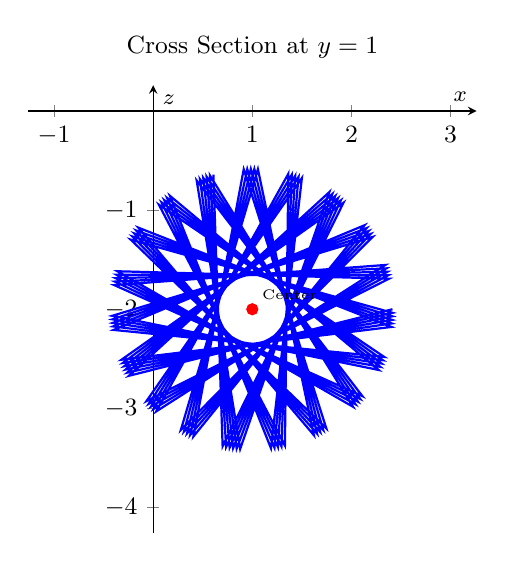
\begin{tikzpicture}
\begin{axis}[
    xlabel={$x$}, ylabel={$z$},
    title={Cross Section at $y=1$},
    axis lines=center,
    enlargelimits=0.3,
    tick label style={font=\small},
    label style={font=\footnotesize},
    title style={font=\small},
    axis equal image
]
% Circle: (x-1)^2 + (z+2)^2 = 2
\addplot[domain=0:360, samples=100, thick, blue] ({1 + sqrt(2)*cos(deg(x))}, {-2 + sqrt(2)*sin(deg(x))});

% Center point
\addplot[only marks, mark=*, red, mark size=2pt] coordinates {(1, -2)};
\node[above right, font=\tiny] at (axis cs:1,-2) {Center};

\end{axis}
\end{tikzpicture}
\end{document}
